%%
%% This is file `prob-mixed.tex',
%% generated with the docstrip utility.
%%
%% The original source files were:
%%
%% probsoln.dtx  (with options: `prob-mixed.tex,package')
%% 
%%  probsoln.dtx
%%  Copyright 2013 Nicola Talbot
%% 
%%  This work may be distributed and/or modified under the
%%  conditions of the LaTeX Project Public License, either version 1.3
%%  of this license of (at your option) any later version.
%%  The latest version of this license is in
%%    http://www.latex-project.org/lppl.txt
%%  and version 1.3 or later is part of all distributions of LaTeX
%%  version 2005/12/01 or later.
%% 
%%  This work has the LPPL maintenance status `maintained'.
%% 
%%  The Current Maintainer of this work is Nicola Talbot.
%% 
%%  This work consists of the files probsoln.dtx and probsoln.ins and the derived files probsoln.sty, sample-exclude.tex, sample.tex, sample2.tex, sample3.tex, sample4.tex, sample5.tex, sample6.tex, sample7.tex, sample8.tex, prob-1stprncp.tex, prob-args.tex, prob-easy.tex, prob-easy2.tex, prob-implicit.tex, prob-mchoice.tex, prob-mixed.tex, prob-newdata.tex, prob-nosoln.tex, prob-probspaces.tex, prob-probspaces2.tex, prob-tabmchoice.tex, prob-verb.tex.
%% 
%% \CharacterTable
%%  {Upper-case    \A\B\C\D\E\F\G\H\I\J\K\L\M\N\O\P\Q\R\S\T\U\V\W\X\Y\Z
%%   Lower-case    \a\b\c\d\e\f\g\h\i\j\k\l\m\n\o\p\q\r\s\t\u\v\w\x\y\z
%%   Digits        \0\1\2\3\4\5\6\7\8\9
%%   Exclamation   \!     Double quote  \"     Hash (number) \#
%%   Dollar        \$     Percent       \%     Ampersand     \&
%%   Acute accent  \'     Left paren    \(     Right paren   \)
%%   Asterisk      \*     Plus          \+     Comma         \,
%%   Minus         \-     Point         \.     Solidus       \/
%%   Colon         \:     Semicolon     \;     Less than     \<
%%   Equals        \=     Greater than  \>     Question mark \?
%%   Commercial at \@     Left bracket  \[     Backslash     \\
%%   Right bracket \]     Circumflex    \^     Underscore    \_
%%   Grave accent  \`     Left brace    \{     Vertical bar  \|
%%   Right brace   \}     Tilde         \~}
%% randomly select 25 problems from derivatives.tex and add to
%% the data set called 'deriv'
%% Display the problems
%% You may need to change \theenumi back here
%% randomly select 25 problems from probspaces.tex and add to
%% the data set called 'spaces'
%% Display the problems
%% You may need to change \theenumi back here
 % This file is public domain
 %
 % These problems are a mixture of essay-style and questions with
 % answers. One of these problems requires the tikz package

\newproblem*{oop}{Describe what is meant by object-oriented
programming.}

\begin{defproblem}{inheritance}
 Describe what is meant by the term \emph{inheritance} in
 object-oriented programming. Use examples.
\end{defproblem}

\begin{defproblem}{weightedcoin}%
  \begin{onlyproblem}
    A coin is weighted so that heads is four times as likely
    as tails. Find the probability that:
    \begin{textenum}
      \item tails appears,
      \item heads appears
    \end{textenum}%
  \end{onlyproblem}%
  \begin{onlysolution}
    Let $p=P(T)$, then $P(H)=4p$. We require $P(H)+P(T)=1$,
    so $4p+p=1$, hence $p=\frac{1}{5}$. Therefore:
    \begin{textenum}
      \item $P(T)=\frac{1}{5}$,
      \item $P(H)=\frac{4}{5}$
    \end{textenum}
  \end{onlysolution}
\end{defproblem}

\begin{defproblem}{validprobspaces}
\begin{onlyproblem}%
Under which of the following functions does
$S=\{a_1,a_2\}$ become a probability space?
\par
\begin{textenum}
\begin{tabular}{ll}
\item $P(a_1)=\frac{1}{3}$, $P(a_2)=\frac{1}{2}$
&
\item\label{validprobspacescorrect1} $P(a_1)=\frac{3}{4}$,
$P(a_2)=\frac{1}{4}$
\\
\item\label{validprobspacescorrect2} $P(a_1)=1$, $P(a_2)=0$
&
\item $P(a_1)=\frac{5}{4}$, $P(a_2)=-\frac{1}{4}$
\end{tabular}
\end{textenum}
\end{onlyproblem}%
\begin{onlysolution}%
\ref{validprobspacescorrect1} and \ref{validprobspacescorrect2}%
\end{onlysolution}
\end{defproblem}

\begin{defproblem}{digraph}
  \begin{onlyproblem}\label{ex:digraph}
  Identify, if any, the sinks and sources of the digraph shown in Figure~\ref{fig:digraph}.

  \begin{figure}[tbh]
    \centering
      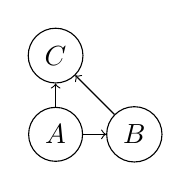
\begin{tikzpicture}[every node/.style={draw,circle}]
         \path (0,0) node (A) {$A$}
               (1,0) node (B) {$B$}
               (0,1) node (C) {$C$};
         \draw[->] (A) -- (B);
         \draw[->] (B) -- (C);
         \draw[->] (A) -- (C);
      \end{tikzpicture}
    \par
    \caption{Digraph for Question~\ref{ex:digraph}}
    \label{fig:digraph}
  \end{figure}
  \end{onlyproblem}
  \begin{onlysolution}
  $A$ is a souce and $C$ is a sink.
  \end{onlysolution}
\end{defproblem}
\endinput
%%
%% End of file `prob-mixed.tex'.
